\subsection{Results}

% add SPIDER benchmark diagram image
\begin{figure}[h]
    \centering
    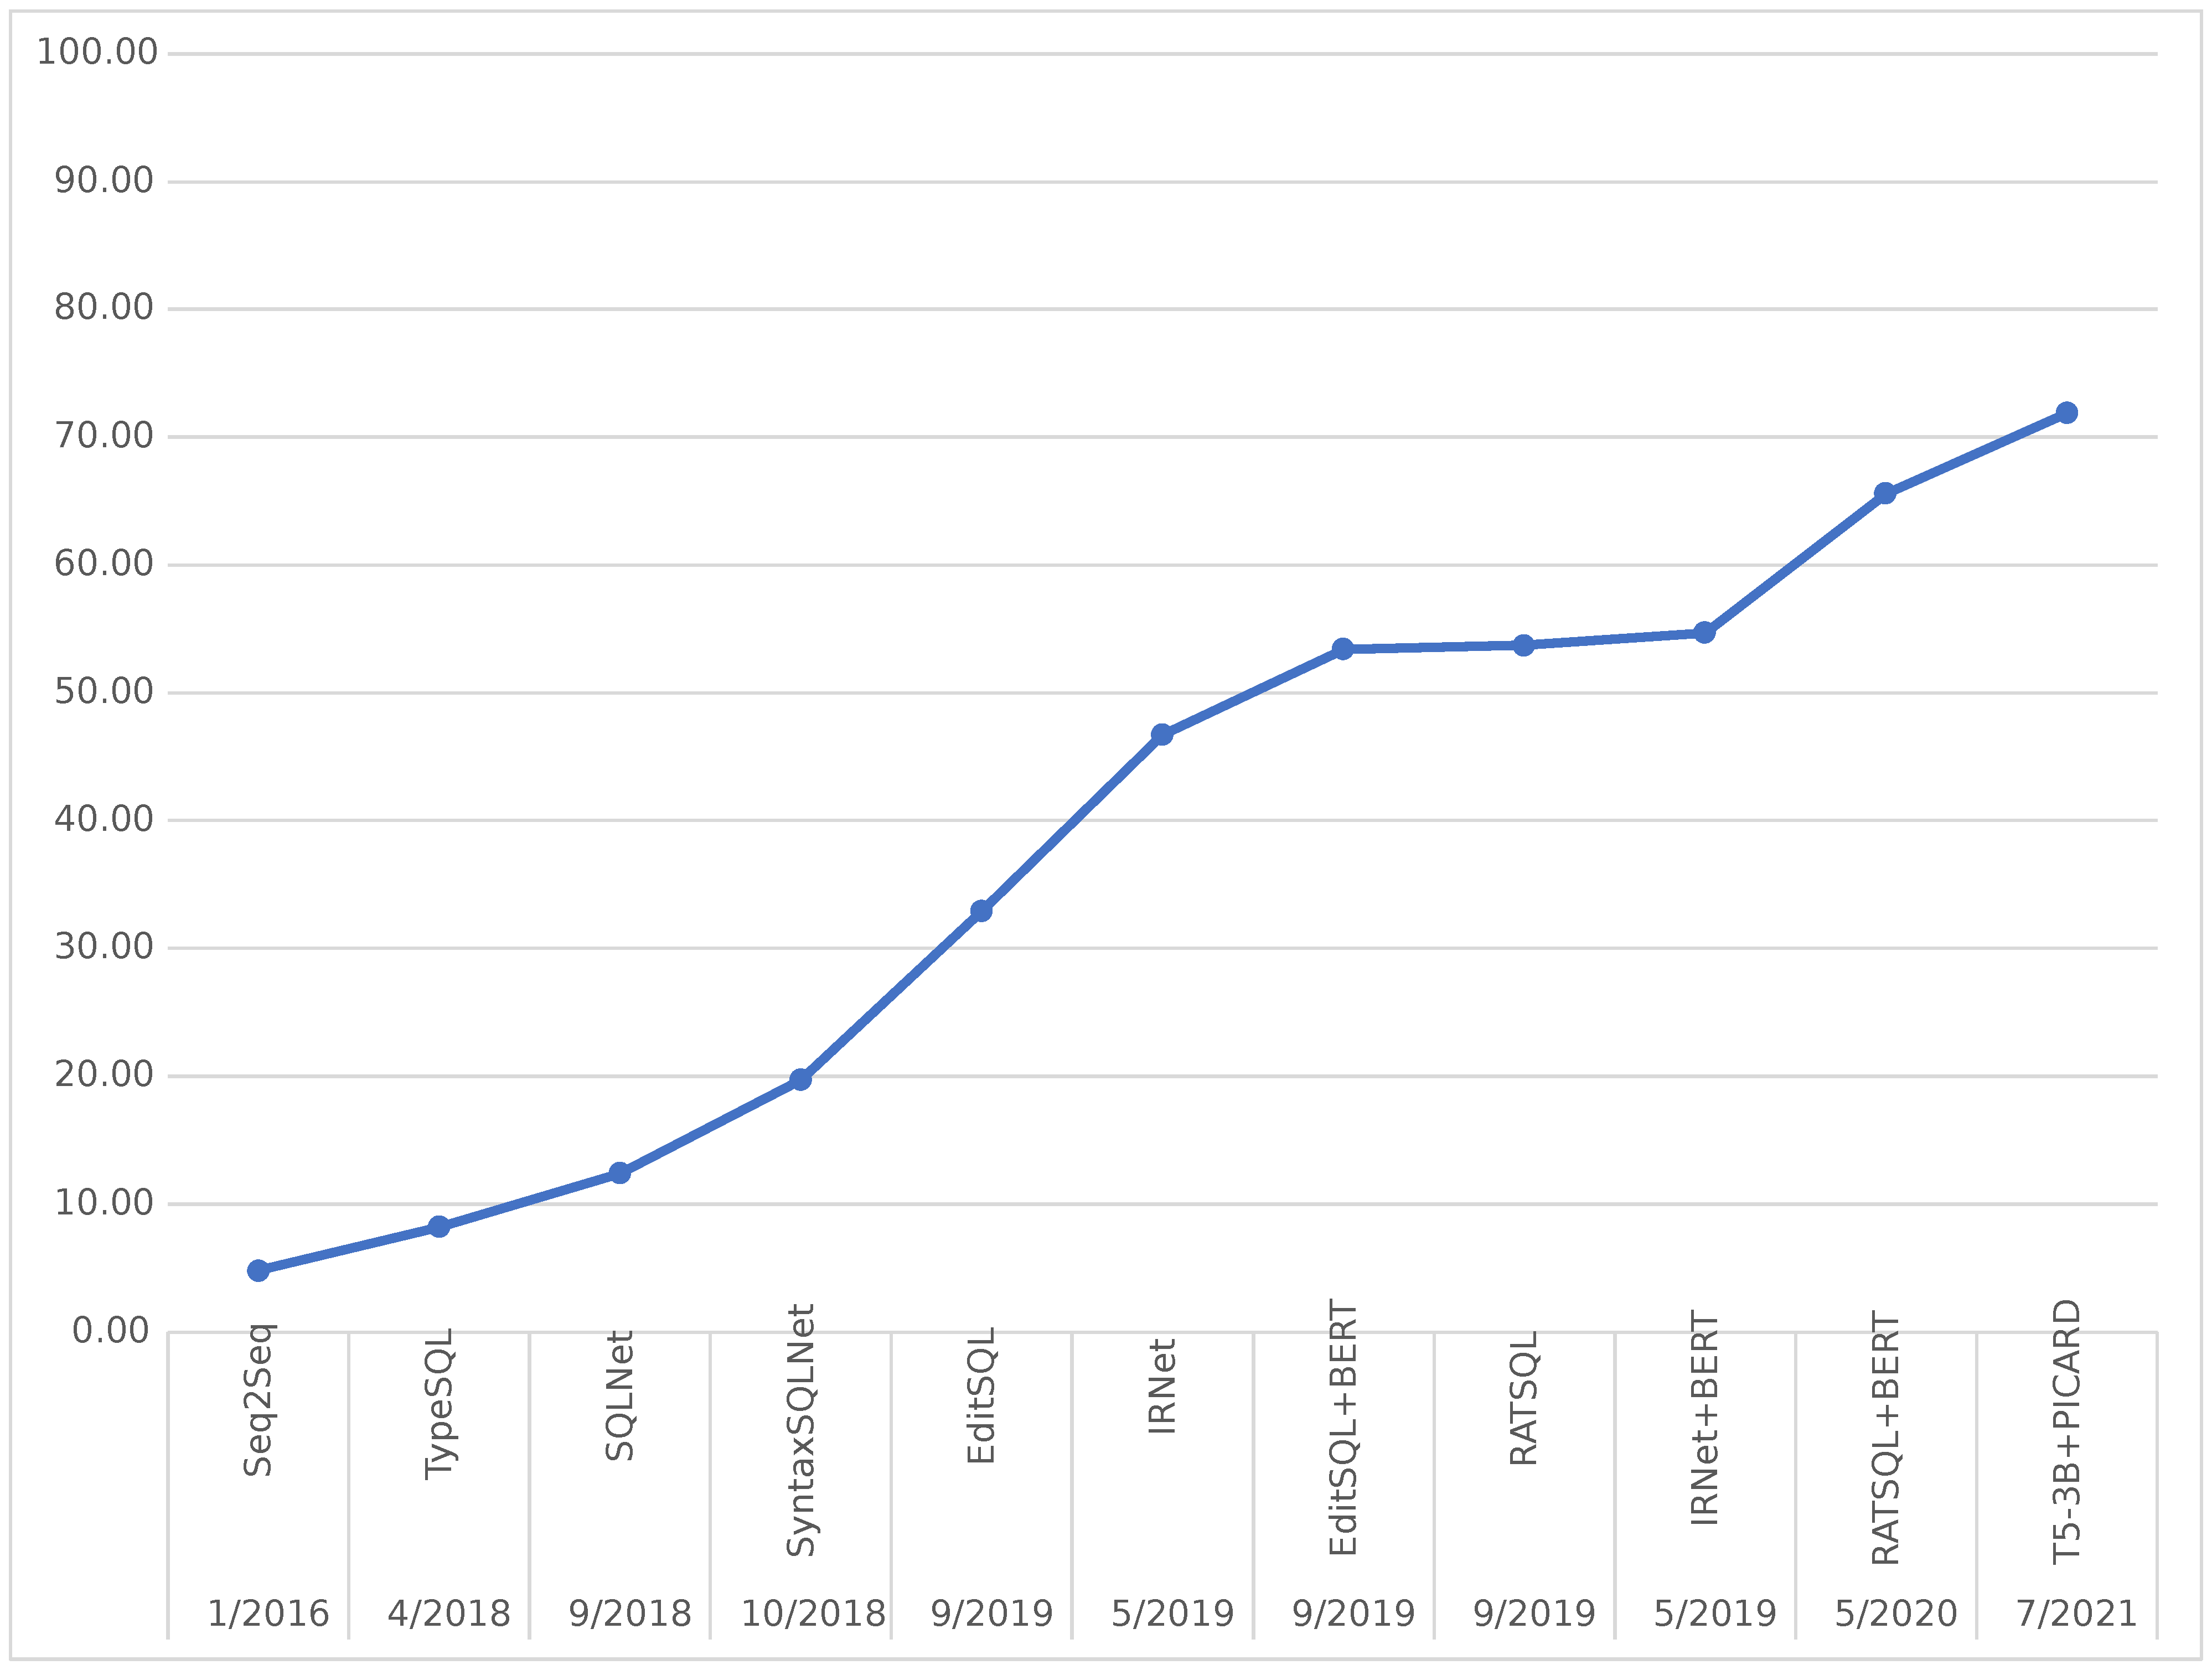
\includegraphics[width=0.99\linewidth]{pics/benchmarkeps}
    \caption{SPIDER benchmark Exact Match Results including our experiments}
    \label{fig:benchmark}
\end{figure}


Throughout this thesis, we have explored the advancements in Text-to-SQL models and their performance on the SPIDER benchmark. Our analysis revealed the significant progress made in the field, with more recent models demonstrating remarkable improvements in generating accurate SQL queries from natural language text.

The integration of powerful pre-trained language models, such as BERT, and cutting-edge architectures like T5 has played a vital role in the observed advancements. The models' ability to learn from limited labeled data, quickly adapt to new tasks or domains, and handle complex SQL queries has been substantially enhanced by employing techniques such as active learning, meta-learning, and multi-task learning.

In the following section, our experiments with ChatGPT-3.5 and ChatGPT-4.0 have showcased their superior performance, achieving scores of 81.30\% and 85.20\% on the SPIDER benchmark, respectively. These results highlight the potential of utilizing the latest huge language models for Text-to-SQL tasks, further pushing the boundaries of what is possible in this domain.

As the field of natural language processing continues to evolve, we can expect even more sophisticated models and techniques to emerge, enabling more accurate and efficient understanding and generation of SQL queries from natural language input. Future research in this area may focus on enhancing the models' ability to handle ambiguous or imprecise input, as well as exploring novel methods to improve their adaptability and generalization capabilities across diverse tasks and domains.

In the next section, we will illustrate different methods for evaluating the performance of such models.